\begin{mybilan}
	
	\begin{center}
		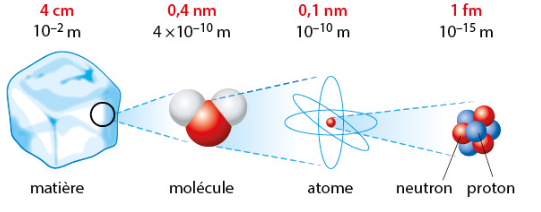
\includegraphics[scale=0.75]{echelle}
	\end{center}

	\begin{itemize}
		\item La taille d'un atome est de l'ordre du dixième de nanomètre, soit $10^{-10} m$.
		\item Le diamètre du noyau est environ \kw{\num{100000} fois plus petit} que celui de l'atome, soit $10^{-15} m$.
		\item L'atome est essentiellement constitué de vide.
		\item La masse des électrons est beaucoup plus faible que celle des nucléons, donc la masse d'un atome est \kw{concentrée dans son noyau}.
	\end{itemize}

	
		
%				%\vspace*{1cm}
		\begin{center}
			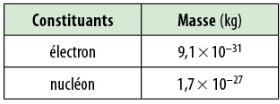
\includegraphics[scale=0.75]{masses}
		\end{center}
	
\end{mybilan}